\chapter{Translation Pipeline} \label{chap:pipeline}
In this chapter, I evaluate the ability of large language models (LLMs) to translate Linear B into Ancient Greek.  
The full pipeline proceeds as follows:

\begin{itemize}[leftmargin=2em]
  \item \textbf{Vocabulary extraction.} Gather every distinct word form attested in the Linear B documents (after cleaning/normalization).
  \item \textbf{Brute-force cognates.} For forms not already covered by our dataset, run the brute-force search against the Ancient Greek lexicon to obtain initial candidates (detailed in Section \ref{sec:bruteforce-cognates}).
  \item \textbf{Candidate aggregation.} For each word, collect possible cognates from: (i) the dataset's suggested cognates, (ii) the trained cognate-matching model's raw output and each decoding mode applied to the new words, and (iii) a version of the cognate matcher retrained on the enlarged set. Duplicates are removed from the candidate set.
  \item \textbf{Auxiliary signals.} Train the Linear-SVM auxiliary classifiers on their labeled sets, then predict part of speech, noun type, and inflection for every word in the corpus.
  \item \textbf{Logograms.} Map logograms to their conventional readings/values and include these as fixed translations.
  \item \textbf{LLM prompting.} For each item, assemble a structured prompt containing: the Linear B form, the deduplicated cognate candidates, auxiliary predictions, and relevant morphological guidance. The LLM is asked to (a) select or propose the most plausible Ancient Greek reconstruction, and (b) provide an English translation.
  If the information provided with the prompt is sufficient, the LLM should be able to reconstruct the right inflection for each term and disambiguate the sentence.
\end{itemize}

\begin{figure}[H]
    \begin{adjustbox}{center}
        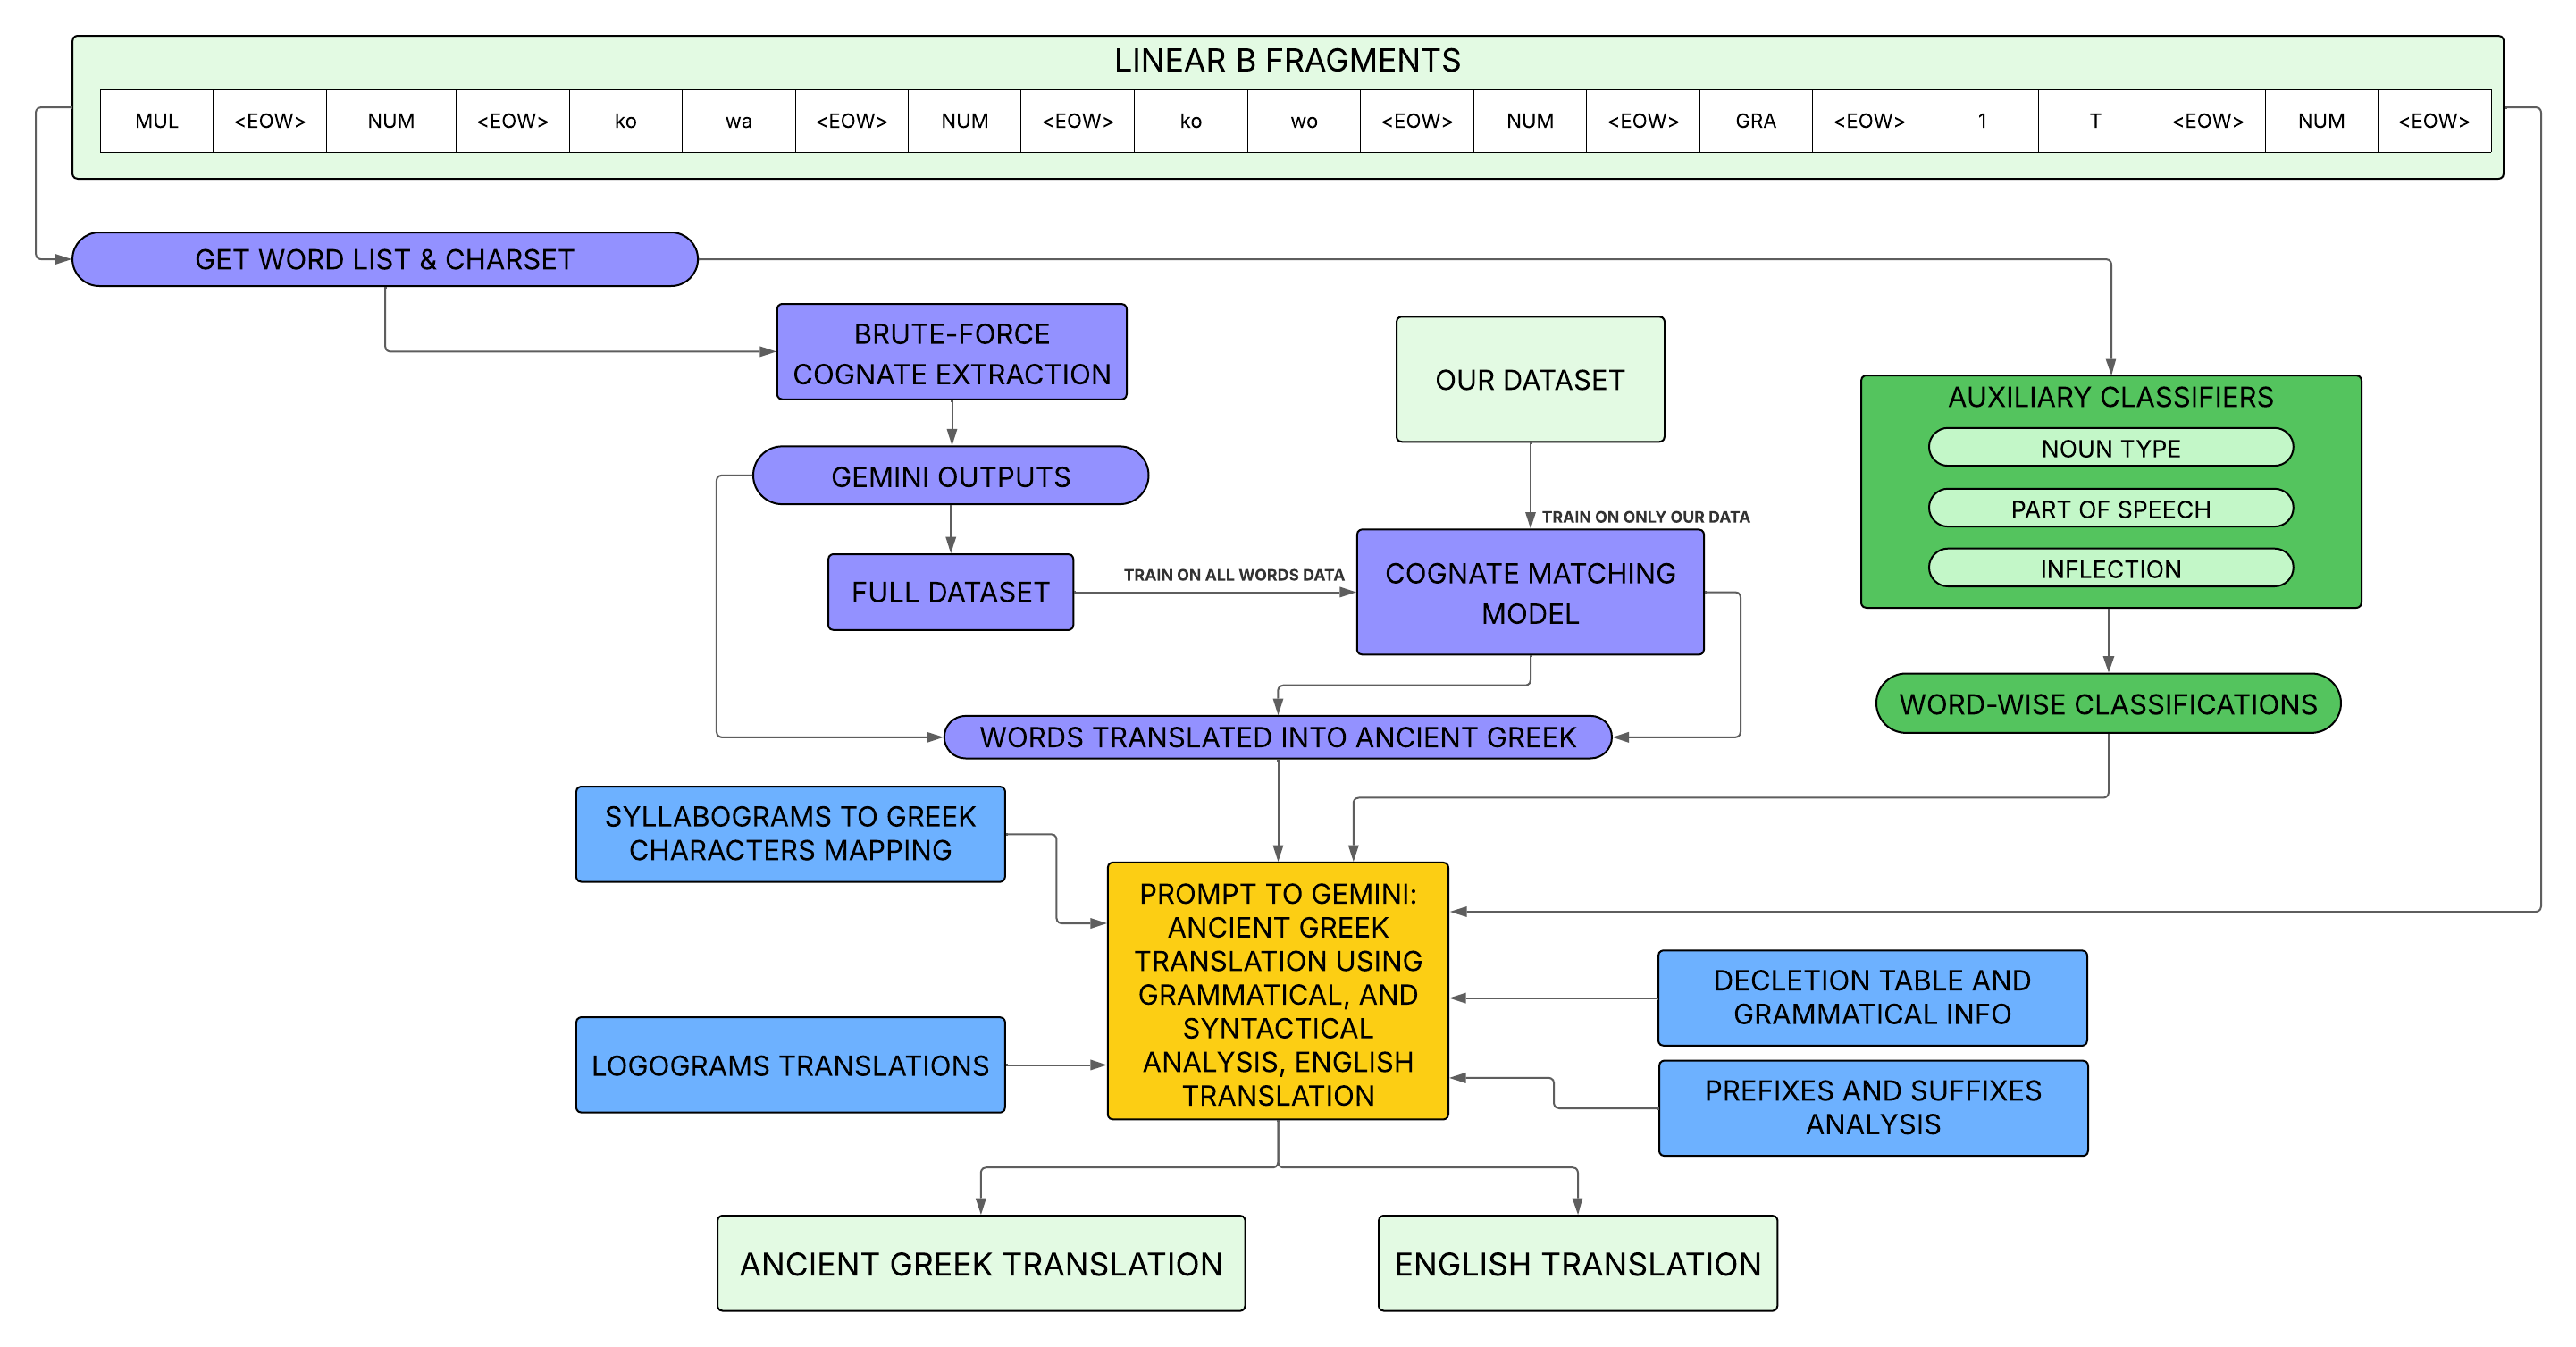
\includegraphics[width=1.2\textwidth]{images/pipeline.png}
    \end{adjustbox}
    \caption{Overview of the translation pipeline from Linear B to Ancient Greek.}
    \label{fig:pipeline}
\end{figure}

\section{Prompt Design} \label{sec:final-prompt}
This time, instead of a single prompt, the information was given to the large language model using a series of structured messages, each with a specific role.

\paragraph{Historical Context}
The first message provided to the model was a simple historical context on Linear B and Ancient Greek relationship.
It underlines the fact that Linear B is an early form of Greek, written with a syllabic script, and its administrative nature.
This message was fixed for all words.

\paragraph{Syllabogram Matching}
The second message contained the Linear B syllabograms and their closest Ancient Greek equivalents, predicted by Luo's model.
It associates to each Linear B syllabogram a list of symbols that could represent it in its Ancient Greek correspondence.
For example, the Linear B syllabogram \textlinb{\Bpa} (pa) is associated with the Ancient Greek letters \textgreek{π}, \textgreek{φ}, and \textgreek{α}, as it usually corresponds to "\textgreek{πα}" or "\textgreek{φα}" syllables.
This was also fixed for all words.

\paragraph{Grammatical Information}
The third message provided auxiliary grammatical information, such as Linear B declension tables, and additional information about adjectives and verbs, like in the prompt described in Section \ref{sec:aux-dataset}.

\paragraph{Task Definition}
The fourth message formalizes the task. The model receives the Linear~B document as a sequence of tokenized word forms; for each word it is given (i) the aggregated set of candidate Ancient Greek cognates, (ii) auxiliary predictions (part of speech, noun type when applicable, and inflection when applicable), and (iii) a completeness label.
The completeness label is derived from the share $p\!\in\![0,1]$ of occurrences marked as "complete" in the corpus and is bucketed at fixed cutoffs:
\emph{Always Complete} ($p=1$), \emph{Mostly Complete} ($p \geq \frac{2}{3}$), \emph{Uncertain} ($\frac{1}{3} < p < \frac{2}{3}$), \emph{Mostly Incomplete} ($0< p \leq \frac{1}{3}$), \emph{Incomplete} ($p=0$).

The prompt instructs the model on how to complete the translation task, the main steps being:
\begin{itemize}
  \item \textbf{Grammatical analysis.} The first step is to analyze the grammatical features of the Linear B document, separating the words into adjectives, nouns, verbs, and adverbs, and reconstructing the inflection of each noun and adjective, as well as the conjugation of each verb.
  \item \textbf{Syntactic analysis.} The second step is to analyze the document's structure by identifying its sentences and distinguishing the subjects, verbs, and objects mentioned in them.
  \item \textbf{Discourse analysis.} The third step is to analyze the discourse, examining subordinate clauses and establishing coherent logical connections.
  \item \textbf{Linguistic authenticity.} The fourth step is to ensure the selection of an Ancient Greek cognate that preserves morphological patterns and is plausible given the corresponding Mycenaean Greek form.
  \item \textbf{Semantic coherence.} The last step is to ensure that the translation is semantically coherent with the administrative nature of the Linear B documents.
\end{itemize}

These are common steps in translation and linguistic analysis, but they are particularly important in this context due to the similarity between Linear B inflected forms.
The LLM is finally asked given some quality assurance criteria, reflecting the needs of the task, and instructed to use the Chain Of Thoughts to technique to reason step by step and refine its translation.

\paragraph{Examples}
The last information given to the model is a series of exampels of translated Linear B fragments.
These examples are selected from a small set of documents provided by Chris Tselentis, together with his Linear B lexicon \cite{tselentis}.

These examples are very short, but they cover a variety of linguistic phenomena and be representative of the administrative purpose of the documents.
The following examples were used:

\begin{enumerate}
  \item \textbf{PY Eb 895+906}: This brief document contains a subordinate clause introduced by a participial form.
  Therefore, it provides key features of Linear B clause structure. \\
  \textbf{Linear B original}: \textlinb{\Ba\Bi\Bqe\Bu} \textlinb{\Be\Bke\Bqe} \textlinb{\Bke\Bke\Bme\Bna} \textlinb{\Bko\Bto\Bna} \textlinb{\Bko\Bto\Bno\Bko} \textlinb{\Bto\Bso\Bde} \textlinb{\Bpe\Bmo} \textlinb{\BPwheat} \textlinb{\BPvolcd} \textlinb{\BNvi}\\
  \textbf{Linear B text}: a-i-qe-u e-ke-qe ke-ke-me-na ko-to-na ko-to-no-o-ko to-so-de pe-mo GRA T 6 \\
  \textbf{Greek translation}: \textgreek{Αἰγεὺς κτοινόοχος ἔχει τε κεκειμένα κτοίνα τοσόνδε σπέρμον ΣΙΤΟΣ Τ 6} \\
  \textbf{English translation}: Aigeus, the plot owner, who owns a communal plot; so much grain: 6 'T' units of wheat. \\
  
  \begin{figure}[H]
    \centering
    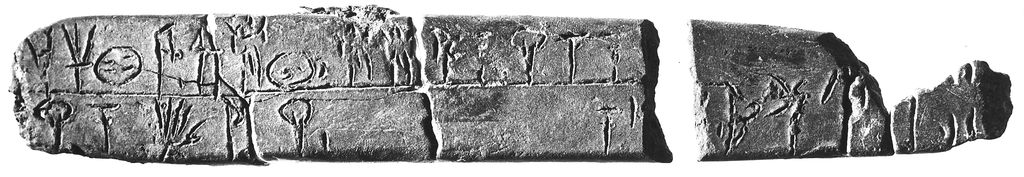
\includegraphics[width=0.7\textwidth]{Images/4901.png} % Adjust width and filename
    \caption{Picture of the original document PY Eb 895+906.}
    \label{fig:example1}
  \end{figure}

  \item \textbf{PY Ta 711}: This fragment is very short as well. It is excerpted from a longer document, whose translation will be fully evaluated in Section \ref{sec:translations}.
  However, it also contains a subordinate clause, introduced here by a particle.
  Moreover, it underscores the importance of grammatical and syntactic analysis, as the subject and the object of the sentence exhibit overlapping inflectional endings. \\
  \textbf{Linear B original}: \textlinb{\Bo\Bwi\Bde} \textlinb{\Bpu\Bke\Bqi\Bri} \textlinb{\Bo\Bte} \textlinb{\Bwa\Bna\Bka} \textlinb{\Bte\Bke} \textlinb{\Bau\Bke\Bwa} \textlinb{\Bda\Bmo\Bko\Bro}\\
  \textbf{Linear B text}: o-wi-de phu-ke-qi-ri o-te wa-na-ka te-ke au-ke-wa da-mo-ko-ro \\
  \textbf{Greek translation}: \textgreek{ὀ-εἶδε Φυγεκλής ὅτε ἄναξ θῆκε Αὐγέαν δάμοκλον} \\
  \textbf{English translation}: Phygekles witnessed when the king appointed Augeus as damoklos. \\

  \begin{figure}[H]
    \centering
    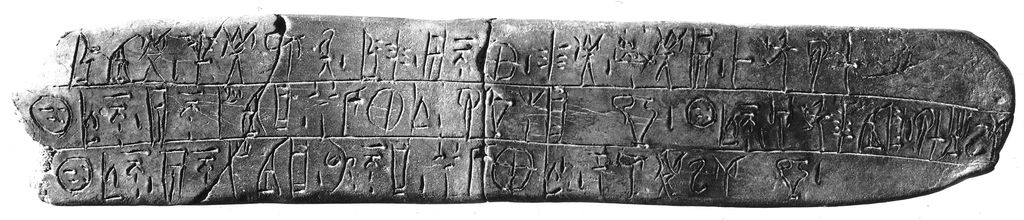
\includegraphics[width=0.8\textwidth]{Images/5350.png} % Adjust width and filename
    \caption{Picture of the original document PY Ta 711.}
    \label{fig:example2}
  \end{figure}

  \item \textbf{PY Ae 303}: This very brief document, like the previous two, illustrates long-distance agreement: the attributive adjective and the noun it modifies stand far apart in the line.
This word-order freedom is common in Ancient Greek and underscores why careful grammatical and logical analysis is essential. \\
  \textbf{Linear B original}: \textlinb{\Bi\Bje\Bro\Bjo} \textlinb{\Bpu\Bro} \textlinb{\Bi\Bje\Bre\Bja} \textlinb{\Bdo\Be\Bra} \textlinb{\Be\Bne\Bka} \textlinb{\Bku\Bru\Bso\Bjo} \textlinb{\BPwoman} \textlinb{\BNx\BNiv}\\
  \textbf{Linear B text}: i-je-ro-jo pu-ro i-je-re-ja do-e-ra e-ne-ka ku-ru-so-jo MUL 14 \\
  \textbf{Greek translation}: \textgreek{Πύλος: ιερείας δούλαι ένεκα χρυσοίο ιεροίο ΓΥΝΗ 14} \\
  \textbf{English translation}: Pylos: slaves of the priestess for the sake of sacred gold, 14 women. \\

  \begin{figure}[H]
    \centering
    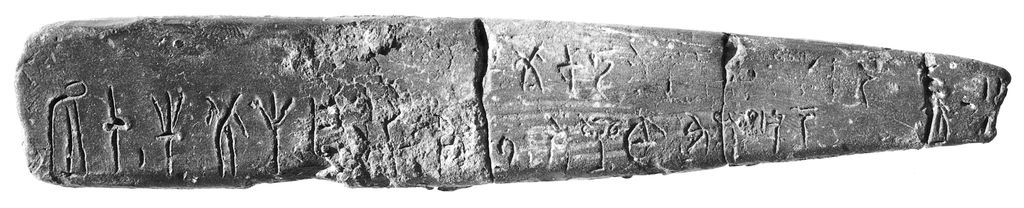
\includegraphics[width=0.7\textwidth]{Images/4684.png} % Adjust width and filename
    \caption{Picture of the original document PY Ae 303.}
    \label{fig:example3}
  \end{figure}

\end{enumerate}

\paragraph{Outputs}
The model is expected to ouput a JSON object with three fields:
\begin{itemize}
  \item \texttt{Ancient Greek}: the reconstructed Ancient Greek translation of the Linear B document.
  \item \texttt{English}: the English translation of the Linear B document.
  \item \texttt{Reasoning}: a detailed reasoning process, following the steps outlined in the task definition, explaining how the model arrived at its translations.
\end{itemize}

\section{Results} \label{sec:translations}
In this section, the outputs of the Translation Pipeline will be presented and compared with existing translations of the same documents, provided by Tselentis' lexicon \cite{tselentis}.
The evaluation will focus on the quality of the Ancient Greek reconstructions and the accuracy of the English translations.
Moreover, errors will be analyzed and the reasoning provided by the model will be assessed to understand the possible causes of mistakes.
A small sample of documents will not be assessed, as it was used as examples in the prompt (see Section \ref{sec:final-prompt}).

\subsection{Evaluated Documents}
The documents selected for evaluation are the following:
\begin{enumerate}[label=(\roman*)]
\item PY Ta 711
\item KN Ra 1540
\item PY Jn 310
\item PY Jn 829
\item KN So 4439
\item KN Sd 4404
\item PY An 657
\item PY TA 641
\item PY Er 312
\item KN Fp 1+31
\item PY Ab 573
\item PY Un 718
\end{enumerate}

The fragments of the documents whose translations were provided by Tselentis are highlighted in \emph{italics}.

\subsubsection{PY Ta 711}
This document was already presented as part of the examples in the prompt to the LLM.
However, only the first fragment was used as an example, while the rest of the document was reserved for evaluation. \\
\textbf{Linear B text}: \textit{o-wi-de phu-ke-qi-ri o-te wa-na-ka te-ke au-ke-wa da-mo-ko-ro} qe-ra-na wa-na-se-wi-ja qo-u-ka-ra ko-ki-re-ja *204VAS 1 qe-ra-na a-mo-te-wi-ja ko-ro-no-we-sa qe-ra-na wa-na-se-wi-ja ku-na-ja qo-u-ka-ra 1 to-qi-de-we-sa *204VAS 1 \\
\textbf{Greek translation}: \textgreek{ὀ-εἶδε Φυγεκλής ὅτε ἄναξ θῆκε Αὐγέαν δάμοκλον. κερανα ϝανασεϝια βουκαρα κοχλιρεια ΣΚΕΥΟΣ 1. κερανα αρμοθηϝια κορωνοϝέσσα. κερανα ϝανασεϝια γυναια βουκαρα 1. τροπιδϝέσσα ΣΚΕΥΟΣ 1.} \\
\textbf{English translation}: Phygekles witnessed when the king appointed Augeus as damoklos. A royal, ox-head-shaped, spiral-decorated krater (vessel): 1. A krater with fittings, with a handle. A royal, female, ox-head-shaped krater: 1. A spiral-designed vessel: 1.

\paragraph{Analysis.}
After the first narrative clause, the document lists four types of vessels.
The LLM correctly reconstructs the context and provides a meaningful and coherent translation.

Let's analyze the four vessel descriptions in detail:
\begin{itemize}
\item The word \textlinb{\Bqe\Bra\Bna} (qe-ra-na) is correctly identified as a noun, and the LLM selects the Ancient Greek cognate \textgreek{κερανα}.
However, the expected form would definitely be \textgreek{κέρνα}, the nominative/accusative plural of \textgreek{κέρνος}, which is used in Ancient Greek to denote a sacred vessel.
\item The word \textlinb{\Bwa\Bna\Bse\Bwi\Bja} (wa-na-se-wi-ja) is correctly identified as an adjective, and the LLM selects an Ancient Greek form that closely echoes the original Linear B word: \textgreek{ϝανασεϝια}, rather than the Ancient Greek \textgreek{αναξια}.
Other adjectives referring to this vessel are \textlinb{\Bqo\Bu\Bka\Bra} (qo-u-ka-ra, "ox-head shaped") and \textlinb{\Bko\Bi\Bre\Bja} (ko-ki-re-ja, "spiral-decorated").
The first is associated with a synthetic compound Ancient Greek form composed of \textgreek{βους} "ox" and \textgreek{καρα} "head", while the second is translated as \textgreek{κοχλιρεια}, an adjective derived from \textgreek{κοχλος}, "spiral-shaped shell", sharing the root with Ancient Greek \textgreek{κοχλιοειδης/κοκλιωδης}.
\item The following vessel is associated with the adjectives \textlinb{\Bko\Bro\Bno\Bwe\Bsa} (ko-ro-no-we-sa), meaning the krater is provided with handles (from Ancient Greek \textgreek{κορωνη}), and \textlinb{\Ba\Bmo\Bte\Bwi\Bja} (a-mo-te-wi-ja), linked to the concept of "fittings" or chariot-related terms (from Ancient Greek \textgreek{αρμος} "joint" and \textgreek{αρμα} "chariot"), even though no fully satisfactory Greek correspondence can be found.
\item The third vessel is again described as royal and ox-head shaped, but the third adjective is \textlinb{\Bku\Bna\Bja} (ku-na-ja), from Ancient Greek \textgreek{γυναια}, "womanly".
\item The last vessel is described as \textlinb{\Bto\Bqi\Bde\Bwe\Bsa} (to-qi-de-we-sa), "spiral-designed", from Ancient Greek \textgreek{τροπιδϝέσσα}, derived from \textgreek{τροπις}, which actually means "keel", and whose connection to spirals is only indirect through the notion of turning or curving, but is also confirmed by Tselentis' lexicon \cite{tselentis}.
\end{itemize}
Overall, the LLM's English translation is quite accurate, while the Ancient Greek reconstruction still retains Linear B features.

Here I report an improved version of the Greek translation, highlighting in red the adjustments. For the English translation, no changes are needed. \\
\textbf{Greek translation}: \textcolor{red}{\textgreek{οἶδε}} \textgreek{Φυγεκλής ὅτε ἄναξ θῆκε Αὐγέαν δάμοκλον.} \textcolor{red}{\textgreek{κέρνα ἀναξία}} \textgreek{βουκάρα} \textcolor{red}{\textgreek{κοχλιοειδή}} \textgreek{ΣΚΕΥΟΣ 1.} \textcolor{red}{\textgreek{κέρνα}} \textgreek{αρμοθήϝια κορωνοϝέσσα}. \textcolor{red}{\textgreek{κέρνα ἀναξία}} \textgreek{γυναίκα βουκάρα 1. τροπιδϝέσσα ΣΚΕΥΟΣ 1.}

\subsubsection{KN Ra 1540}
This document is a very short inventory entry of a single item: swords. \\
\textbf{Linear B text}: \textit{to-sa pa-ka-na PUG 50} \\
\textbf{Greek translation}: \textgreek{τόσα φάσγανα ΦΑΣΓΑΝΑ 50.} \\
\textbf{English translation}: So many swords: 50 SWORDS.
\paragraph{Analysis.}
In this case, the LLM correctly reconstructs the whole document, due to its simplicity.
The words \textlinb{\Bto\Bsa} (to-sa) and \textlinb{\Bpa\Bka\Bna} (pa-ka-na) are correctly identified as a quantifier and a noun, respectively.
They are translated into their corresponding Ancient Greek cognates: \textgreek{τόσα} and \textgreek{ϝάσγανα}, the accusative plural of \textgreek{ϝάσγανον}, "sword".
The English translation is also accurate, therefore no changes are needed.

\subsubsection{PY Jn 310}
Tselentis provides a translation for only a fragment of this document, which is quite long.
However, the LLM appears able to handle the entire text quite well, thanks to its repetitive structure. \\
\textbf{Linear B text}: a-ke-re-wa [...] ka-ke-we ta-ra-si-ja e-ko-te ti-qa-jo AES M 1 N 2 qe-ta-wo AES M 1 N 2 ai-so-ni-jo AES M 1 N 2 ta-mi-je-u AES M 1 N 2 e-u-ru-wo-ta AES M 1 N 2 e-u-do-no AES M 1 N 2 po-ro-u-te-u AES M 1 N 2 wi-du-wa-ko AES M 1 N 2 to-so-de a-ta-ra-si-jo ka-ke-we [...] pa-qo-si-jo 1 ke-we-to 1 [...] 1 [...] pe-ta-ro 1 to-so-de do-e-ro ke-we-to-jo 1 i-wa-ka-o 1 pa-qo-si-jo-jo 1 po-ro-u-te-wo 1 a [...] \textit{po-ti-ni-ja-we-jo ka-ke-we ta-ra-si-ja e-ko-te} i-ma-di-jo [...] AES M 3 tu-ke-ne-u AES M 3 AES M 3 i-wa-ka AES M 3 a-ta-ra-si-jo phu-si-ja-ko 1 \\
\textbf{Greek translation}: \textgreek{Ἀγρεϝα [...] χαλκεϝες ταλανσία ἔχοντες: Τιθαιος ΧΑΛΚΟΣ M 1 N 2, Κεταϝος ΧΑΛΚΟΣ M 1 N 2, Αἰσώνιος ΧΑΛΚΟΣ M 1 N 2, Ταμιεύς ΧΑΛΚΟΣ M 1 N 2, Εὐρυϝότας ΧΑΛΚΟΣ M 1 N 2, Εὔδονος ΧΑΛΚΟΣ M 1 N 2, Πλουτεύς ΧΑΛΚΟΣ M 1 N 2, Ϝιδυϝακος ΧΑΛΚΟΣ M 1 N 2. Τόσοςδε ἀταλανσίοι χαλκεϝες [...]: Παμφίσιος 1, Κηϝετος 1, [...] 1, [...] 1, Πέταλος 1. Τόσοςδε δοῦλοι: Κηϝετοιο 1, Ἰϝακαο 1, Παμφισίοιο 1, Πλουτέϝος 1. Ἀ [...] Ποτνιάϝειοι χαλκεϝες ταλανσία ἔχοντες: Ἱμαδιος [...] ΧΑΛΚΟΣ M 3, Τυχενεύς ΧΑΛΚΟΣ M 3, ΧΑΛΚΟΣ M 3, Ἰϝακα ΧΑΛΚΟΣ M 3. Ἀταλανσίοι: Φυσίαρχος 1.} \\
\textbf{English translation}: Agrewa: [...] bronze-smiths having allotment: Tithaios: BRONZE M 1 N 2, Ketawo: BRONZE M 1 N 2, Aisonios: BRONZE M 1 N 2, Tamieus: BRONZE M 1 N 2, Eurywotas: BRONZE M 1 N 2, Eudonos: BRONZE M 1 N 2, Plouteus: BRONZE M 1 N 2, Widuwako: BRONZE M 1 N 2. Total bronze-smiths without allotment [...]: Pamphisios 1, Kewetos 1, [...] 1, [...] 1, Petalos 1. Total slaves: Of Kewetos 1, Of Iwaka 1, Of Pamphisios 1, Of Plouteus 1. A [...] Potnia-related bronze-smiths having allotment: Himadios [...] BRONZE M 3, Tucheneus: BRONZE M 3, BRONZE M 3, Iwaka: BRONZE M 3. Without allotment: Physiarchos 1.

\paragraph{Analysis.}
This document is an administrative record from the site of Pylos, listing bronze-smiths, their allotments of bronze, and associated personnel (slaves).
It is structured into several sections based on the status and affiliation of the craftsmen.
Most words occurring in the document are proper nouns, for which the Ancient Greek correspondence is a simple transliteration.
The most notable common words are:
\begin{itemize}
\item \textlinb{\Bka\Bke\Bwe} (ka-ke-we), "bronze-smith", from Ancient Greek \textgreek{χαλκεύς}, correctly identified as a noun by the LLM and transliterated in a form preserving the digamma (\textgreek{χαλκεϝες} rather than \textgreek{χαλκεῖς}).
\item \textlinb{\Bta\Bra\Bsi\Bja} (ta-ra-si-ja), "allotment", from Ancient Greek \textgreek{ταλανσία}, also correctly identified as a noun.
It shares its root with \textgreek{τάλαντον}, "talent", a unit of weight (and later currency), with the sense of "allotment" deriving from a weight of metal assigned to a worker.
\item \textlinb{\Be\Bko\Bte} (e-ko-te), "having", from Ancient Greek \textgreek{ἔχοντες}, the nominative plural masculine present active participle of \textgreek{ἔχω}, "to have".
Another straightforward form is \textlinb{\Bdo\Be\Bro} (do-e-ro), from Ancient Greek \textgreek{δοῦλοι}, the nominative plural masculine of \textgreek{δοῦλος}, "slave".
\item Both \textlinb{\Bto\Bso\Bde} (to-so-de) and \textlinb{\Ba\Bta\Bra\Bsi\Bjo} (a-ta-ra-si-jo) are interpreted as nominative plural adjectives referring to the bronze-smiths.
The former means "so many" or "total", from Ancient Greek \textgreek{τοσόσδε}, while the latter means "without allotment", from Ancient Greek \textgreek{ἀταλανσίος}, built from the negative prefix \textgreek{ἀ-} and \textgreek{ταλανσία}, "allotment".
\item The translation of \textlinb{\Bpo\Bti\Bni\Bja\Bwe\Bjo} (po-ti-ni-ja-we-jo) is problematic in this context.
While the LLM interprets it as a nominative plural associated with the bronze-smiths, Tselentis gives it a locative neuter value, linking it to the initial word \textlinb{\Ba\Bke\Bre\Bwa} (a-ke-re-wa), a toponym.
Accordingly, while the LLM's rendering remains vague, Tselentis' proposal is to read it as "at the place of Potnia", associating it with \textgreek{ποτνιάδειον}.
\end{itemize}

The LLM's English translation is quite accurate, although it reflects the issue with the word "po-ti-ni-ja-we-jo".
For both translations, I report an improved version below, highlighting in red the adjustments and in blue the actual mistakes. \\
\textbf{Greek translation}: \textgreek{Ἀγρεϝα [...]} \textcolor{red}{\textgreek{χαλκεῖς}} \textgreek{ταλανσία ἔχοντες: Τιθαιος ΧΑΛΚΟΣ M 1 N 2, Κεταϝος ΧΑΛΚΟΣ M 1 N 2, Αἰσώνιος ΧΑΛΚΟΣ M 1 N 2, Ταμιεύς ΧΑΛΚΟΣ M 1 N 2, Εὐρυϝότας ΧΑΛΚΟΣ M 1 N 2, Εὔδονος ΧΑΛΚΟΣ M 1 N 2, Πλουτεύς ΧΑΛΚΟΣ M 1 N 2, Ϝιδυϝακος ΧΑΛΚΟΣ M 1 N 2.} \textcolor{red}{\textgreek{Τοσοίδε}} \textgreek{ἀταλανσίοι} \textcolor{red}{\textgreek{χαλκεῖς}} \textgreek{[...]: Παμφίσιος 1, Κηϝετος 1, [...] 1, [...] 1, Πέταλος 1.} \textcolor{red}{\textgreek{Τοσοίδε}} \textgreek{δοῦλοι: Κηϝετοιο 1,} \textcolor{red}{\textgreek{Ἰϝακας}} \textgreek{1, Παμφισίοιο 1, Πλουτέϝος 1. Ἀ [...]} \textcolor{blue}{\textgreek{ποτνιάδειον}} \textcolor{red}{\textgreek{χαλκεῖς}} \textgreek{ταλανσία ἔχοντες: Ἱμαδιος [...] ΧΑΛΚΟΣ M 3, Τυχενεύς ΧΑΛΚΟΣ M 3, ΧΑΛΚΟΣ M 3, Ἰϝακα ΧΑΛΚΟΣ M 3. Ἀταλανσίοι: Φυσίαρχος 1.} \\
\textbf{English translation}: Agrewa: [...] bronze-smiths having allotment: Tithaios: BRONZE M 1 N 2, Ketawo: BRONZE M 1 N 2, Aisonios: BRONZE M 1 N 2, Tamieus: BRONZE M 1 N 2, Eurywotas: BRONZE M 1 N 2, Eudonos: BRONZE M 1 N 2, Plouteus: BRONZE M 1 N 2, Widuwako: BRONZE M 1 N 2. Total bronze-smiths without allotment [...]: Pamphisios 1, Kewetos 1, [...] 1, [...] 1, Petalos 1. Total slaves: Of Kewetos 1, Of Iwaka 1, Of Pamphisios 1, Of Plouteus 1. A [...] \textcolor{blue}{At the place of Potnia}: bronze-smiths having allotment: Himadios [...] BRONZE M 3, Tucheneus: BRONZE M 3, BRONZE M 3, Iwaka: BRONZE M 3. Without allotment: Physiarchos 1.

\subsubsection{PY Jn 829}
PALLE PALLE...

\subsubsection{KN So 4439}
